\begin{multicols}{3}[\section{NFC}]

\rhead{Mirko Grothe, Jan Selig}
\lfoot{14.05.2016}

\newrefsegment

\begin{tabular}{p{2,1 cm}p{2.7 cm}}
\textbf{Steckbrief}& \\
\end{tabular}
\rowcolors{1}{mobile}{}
\begin{tabular}{p{2,1 cm}p{2.7 cm}}
      Einsatz seit & 2002\\
      \hline
      Frequenz"-bereich  & \SI{13.56}{\mega\hertz}\\
      \hline
      Datenrate & \SI{424}{kBit/s}\\
      \hline
      Verbreitung & gering\\
      \hline
      Reichweite & \SI{4}{cm}\\
      \hline
      Entwickelt von & Sony und Philips \\
      \hline
      Spezifiziert durch & NFC Forum \\
      \hline
      Technologie & RFID \\
      \hline
      Standardisierung & ISO/IEC 18000-3 \\
     \hline
      Modulation & Phasen Jitter Modulation \\
\end{tabular}
\par


\subsection*{Überblick}
\begin{wrapfigure}{r}{0.4\linewidth} 
\vspace{-20pt} 
\begin{center} 
\hspace{-20pt} 
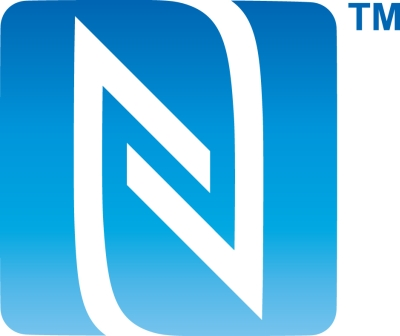
\includegraphics[width=0.7\linewidth]{Kapitel/NFC/Grafiken/Logo.jpg} 
\end{center} 
\vspace{-15pt} 
\end{wrapfigure} 


\textbf{N}ear \textbf{F}ield \textbf{C}ommunication\footnote{NFC {http://nfc-forum.org//}} (z.dt. Nahfeldkommunikation, Abkürzung NFC) ist ein internationaler Übertragungsstandard zum kontaktlosen Austausch von Daten zwischen zwei Geräten. Aufgrund der geringen Reichweite und der niedrigen Übertragungsrate ist NFC nicht für das Senden umfangreicher Daten geeignet. Stattdessen ist NFC auf Dienste ausgelegt, bei denen ein Transfer geringer Datenmengen über kurze Reichweiten initiiert wird, ohne das bei jedem Verbindungsaufbau eine zeitintensive Kopplung erforderlich ist.
Die Datenübertragung ist intuitiv und kann daher bei entsprechender Konfiguration automatisch gestartet werden, sobald ein NFC fähiges Gerät in Reichweite ist.~\cite{nfc.1,nfc.2,nfc.12}


\subsection*{Technische Erläuterungen}
NFC wurde gezielt für eine Übertragung geringer Datenmengen mit schnellem Verbindungsauf und -abbau entwickelt. Dies wird realisiert, indem der Datentransfer zwischen zwei NFC fähigen Geräten automatisch initiiert wird, sobald diese in Reichweite sind. Um unbeabsichtigte Verbindungen oder ein Abhören der zu übermittelnden Daten zu verhindern, ist die Übertragung mit NFC nur in geringer Reichweite im Zentimeterbereich möglich. Damit kann eine Kontaktaufnahme als Zustimmung zu einer Datentransaktion gewertet werden. Bei sicherheitskritischen Transaktionen wie Kreditkartenzahlungen erfolgt die Kommunikation zusätzlich verschlüsselt.

Jedes NFC Gerät unterstützt zwei Betriebsmodi. Im \textit{passiven Modus} wird das Senden und Empfangen von Daten von einem anderen aktiven Gerät initiiert und gesteuert. Das passive Gerät kann hierbei ausgeschaltet sein. 
Im \textit{aktiven Modus} kann ein Gerät zusätzlich zur passiven Funktion einen Datentransfer selbst veranlassen. Sind beide Geräte im aktiven Modus, so spricht man auch vom sogenannten Peer-to-Peer-Modus, da ein Datenaustausch in Form eines Dialogs möglich ist. 

Des Weiteren gibt es sogenannte NFC Tags; diese besitzen im Gegensatz zu NFC Geräten keine eigene Stromversorgung und können äquivalent zu ausgeschalteten Geräten nur im passiven Modus arbeiten. Darüber hinaus können sie, anders als NFC Geräte, nicht gleichzeitig Daten senden und empfangen.

NFC nutzt die RFID Technologie (radio-frequency identification), die in Abb. \ref{fig:nfc.RFID} dargestellt ist. Diese ist ein Sender-Empfänger-System zum automatischen und berührungslosen Identifizieren von Objekten über Funkwellen mit einer Frequenz von 13.56~MHz~\cite{nfc.9}. Jedes NFC Gerät (nicht NFC Tags) kann sowohl die Rolle des Senders, als auch die des Empfängers übernehmen. Mit seiner Peer-to-Peer-Funktion grenzt sich NFC zur RFID Technologie ab, bei der nur eine Kommunikation zwischen aktivem Sender und passivem Empfänger möglich ist. 

\begin{Figure}
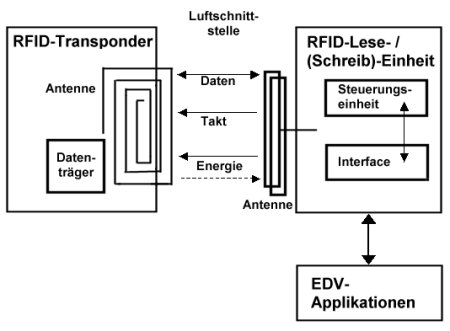
\includegraphics[width=\linewidth]{Kapitel/NFC/Grafiken/RFID.jpeg}
\captionof{figure}{RFID Technologie~\cite{nfc.13}}
\label{fig:nfc.RFID}
\end{Figure}

Ein anfragendes Gerät erzeugt mittels einer Spule ein elektromagnetisches Wechselfeld mit einer Trägerfrequenz von 13,56~MHz. Unterschreitet es dabei den maximalen Senderadius zu einem anderen Gerät, so induziert es über eine Spule im Stromkreis des empfangenden Gerätes eine Spannung. Weil das Magnetfeld aufgrund der Wechselspannung nicht konstant ist, fungiert es für das empfangende Gerät als konstante Energiequelle, solange letzteres sich innerhalb dessen Sendereichweite befindet. Aus diesem Grund kann ein Gerät im passiven Modus von seiner eigenen Energieversorgung getrennt sein und ein NFC Tag ohne eigene Energiequelle auskommen.

Über die sogenannte induktive Kopplung zwei benachbarter elektrischer Stromkreise erfolgt neben der Energieübertragung auch die Kommunikation der beiden Geräte. Die Daten werden über das Magnetfeld per Phasen Jitter Modulation von dem anfragenden Gerät an das empfangende Gerät gesendet. 

\begin{Figure}
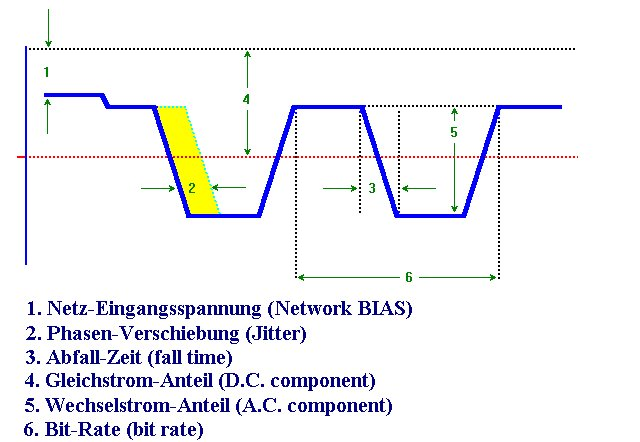
\includegraphics[width=\linewidth]{Kapitel/NFC/Grafiken/PJM.jpg}
\captionof{figure}{Phasen Jitter Modulation~\cite{nfc.14}}
\label{fig:nfc.PJM}
\end{Figure}

Die PJM (Abb. \ref{fig:nfc.PJM}) ist eine abgeschwächte Form der Phasenmodulation, bei der vom sendenden Gerät nur sehr kleine Änderungen an der Phase des Trägersignals vorgenommen werden. Während der unmodulierte Teil des Signals zur Energieversorgung des Empfängers dient, demoduliert und interpretiert dieser den geringen modulierten Anteil des Signals durch Vergleichen mit dem unmodulierten Anteil. 

Bei der Datenübertragung vom Empfänger zurück zum anfragenden Gerät bedient sich Ersterer der modulierten Rückstreuung. Hierbei reflektiert der Empfänger das empfangene Signal mit gleicher Trägerfrequenz und gleichzeitig veränderten Amplituden (Amplituden-Modulation). Dies wird durch kurzeitiges Ändern der Impedanz der Empfängerspule realisiert. Durch Demodulation und Interpretation der veränderten Amplituden des zurückgestreuten Signals erhält das anfragende Gerät die Antwort des empfangenden Gerätes.~\cite{nfc.3,nfc.4,nfc.5,nfc.6,nfc.7,nfc.8}


\subsection*{Einsatz}
\begin{itemize}
\item Kontaktlose Datenübertragung über kurze Distanzen
\item Potentielle Ablösung von Kreditkarten und Schlüsseln aufgrund eines schnellen Verbindungsaufbaus
\item Wasserdichte Konstruktionen der Geräte möglich
\item Mobile Payment zum kontaktlosen Bezahlen mit NFC fähigen Kreditkarten oder Smartphones
\item Schlüsselkarten zum Öffnen von Türen und Schranken
\item Digitale Eintritts- und Fahrkarten
\item Chips zur Arbeitszeiterfassung
\item Pairing zweier Geräte über Bluetooth
\item Bereitstellen von Terminals, die Informationen versenden~\cite{nfc.1,nfc.2,nfc.10}
\end{itemize}
\end{multicols}
\newpage

\section*{Historische Entwicklung}
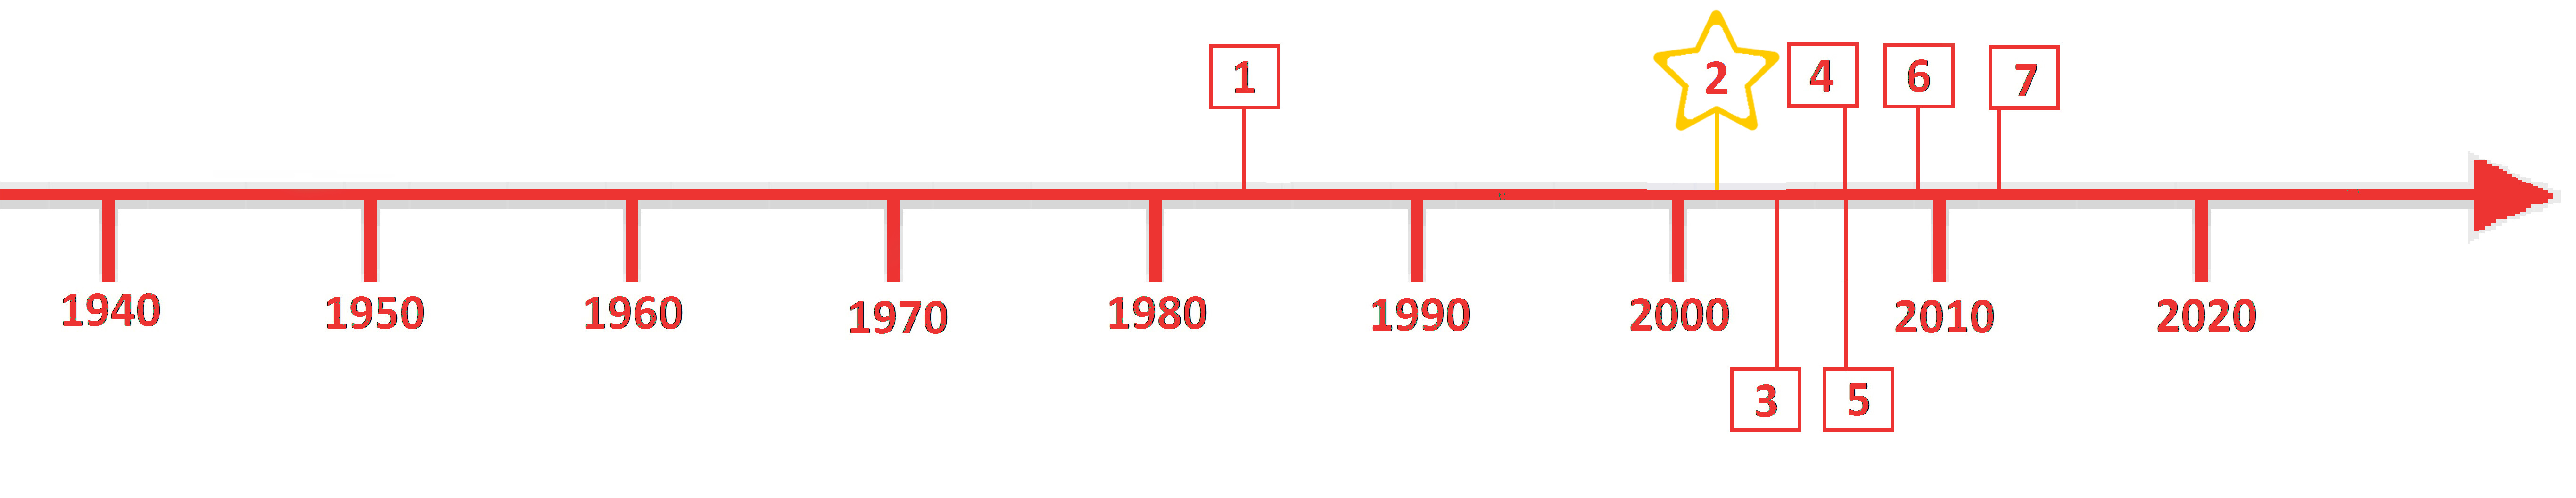
\includegraphics[width=\textwidth]{Kapitel/NFC/Grafiken/Zeitstrahl2}
\par
\noindent
\rowcolors{2}{}{mobile}
\begin{tabular}{p{0.5 cm}p{1.5 cm}p{15.55 cm}}
	\hline
	Nr. & Datum & Entwicklungsschritte~\cite{nfc.1}\\
	\hline
	1 & 1983 & Das erste Patent mit der Abkürzung „RFID“ wird auf Charles Walton ausgestellt.\\
	\hline
	2 & 2002 & Sony und Philips einigen sich auf eine technische Spezifikation.\\
	\hline
	3 & 2004 & Nokia, Philips und Sony etablieren das Near Field Communication (NFC) Forum.\\
	\hline
	4 & 2006 & Erste Spezifikation für NFC-Tags wird veröffentlicht.\\
	\hline
	5 & 2006 & Nokia präsentiert das erste NFC-fähige Mobiltelefon.\\
	\hline
	6 & 2009 & Das NFC-Forum veröffentlicht Peer-to-Peer-Standards.\\
	\hline
	7 & 2012 & Einführung von girogo.\\
	\hline
\end{tabular}
\par
\begin{multicols}{3}

\subsection*{Anbieter und Gremien}
Die 2002 von \textit{Philips} und \textit{Sony} entwickelte Nahfeldkommunikation wird durch die öffentliche Plattform \textit{NFC Forum} spezifiziert. Die Spezifikationen umfassen Standards für die Gerätearchitektur von NFC Geräten und die bei der Kommunikation verwendeten Protokolle.

Seit Anfang 2012 haben in Deutschland Kreditkarten von \textit{Visa} (payWave) und MasterCard (PayPass) einen NFC Chip verbaut. Damit können bei kooperierenden Händlern Beträge bis maximal 25 Euro ohne PIN Abfrage bezahlt werden. Sparkassen und Volksbanken bieten mit ihrer Girocard (girogo (Abb.~\ref{fig:nfc.girogo})) ebenfalls eine NFC Funktion zum kontaktlosen Bezahlen.
Studentenausweise, mit denen man kontaktlos bezahlen kann und auch der neue Personalausweis, enthalten in der Regel noch RFID- statt NFC Chips.

\begin{Figure}
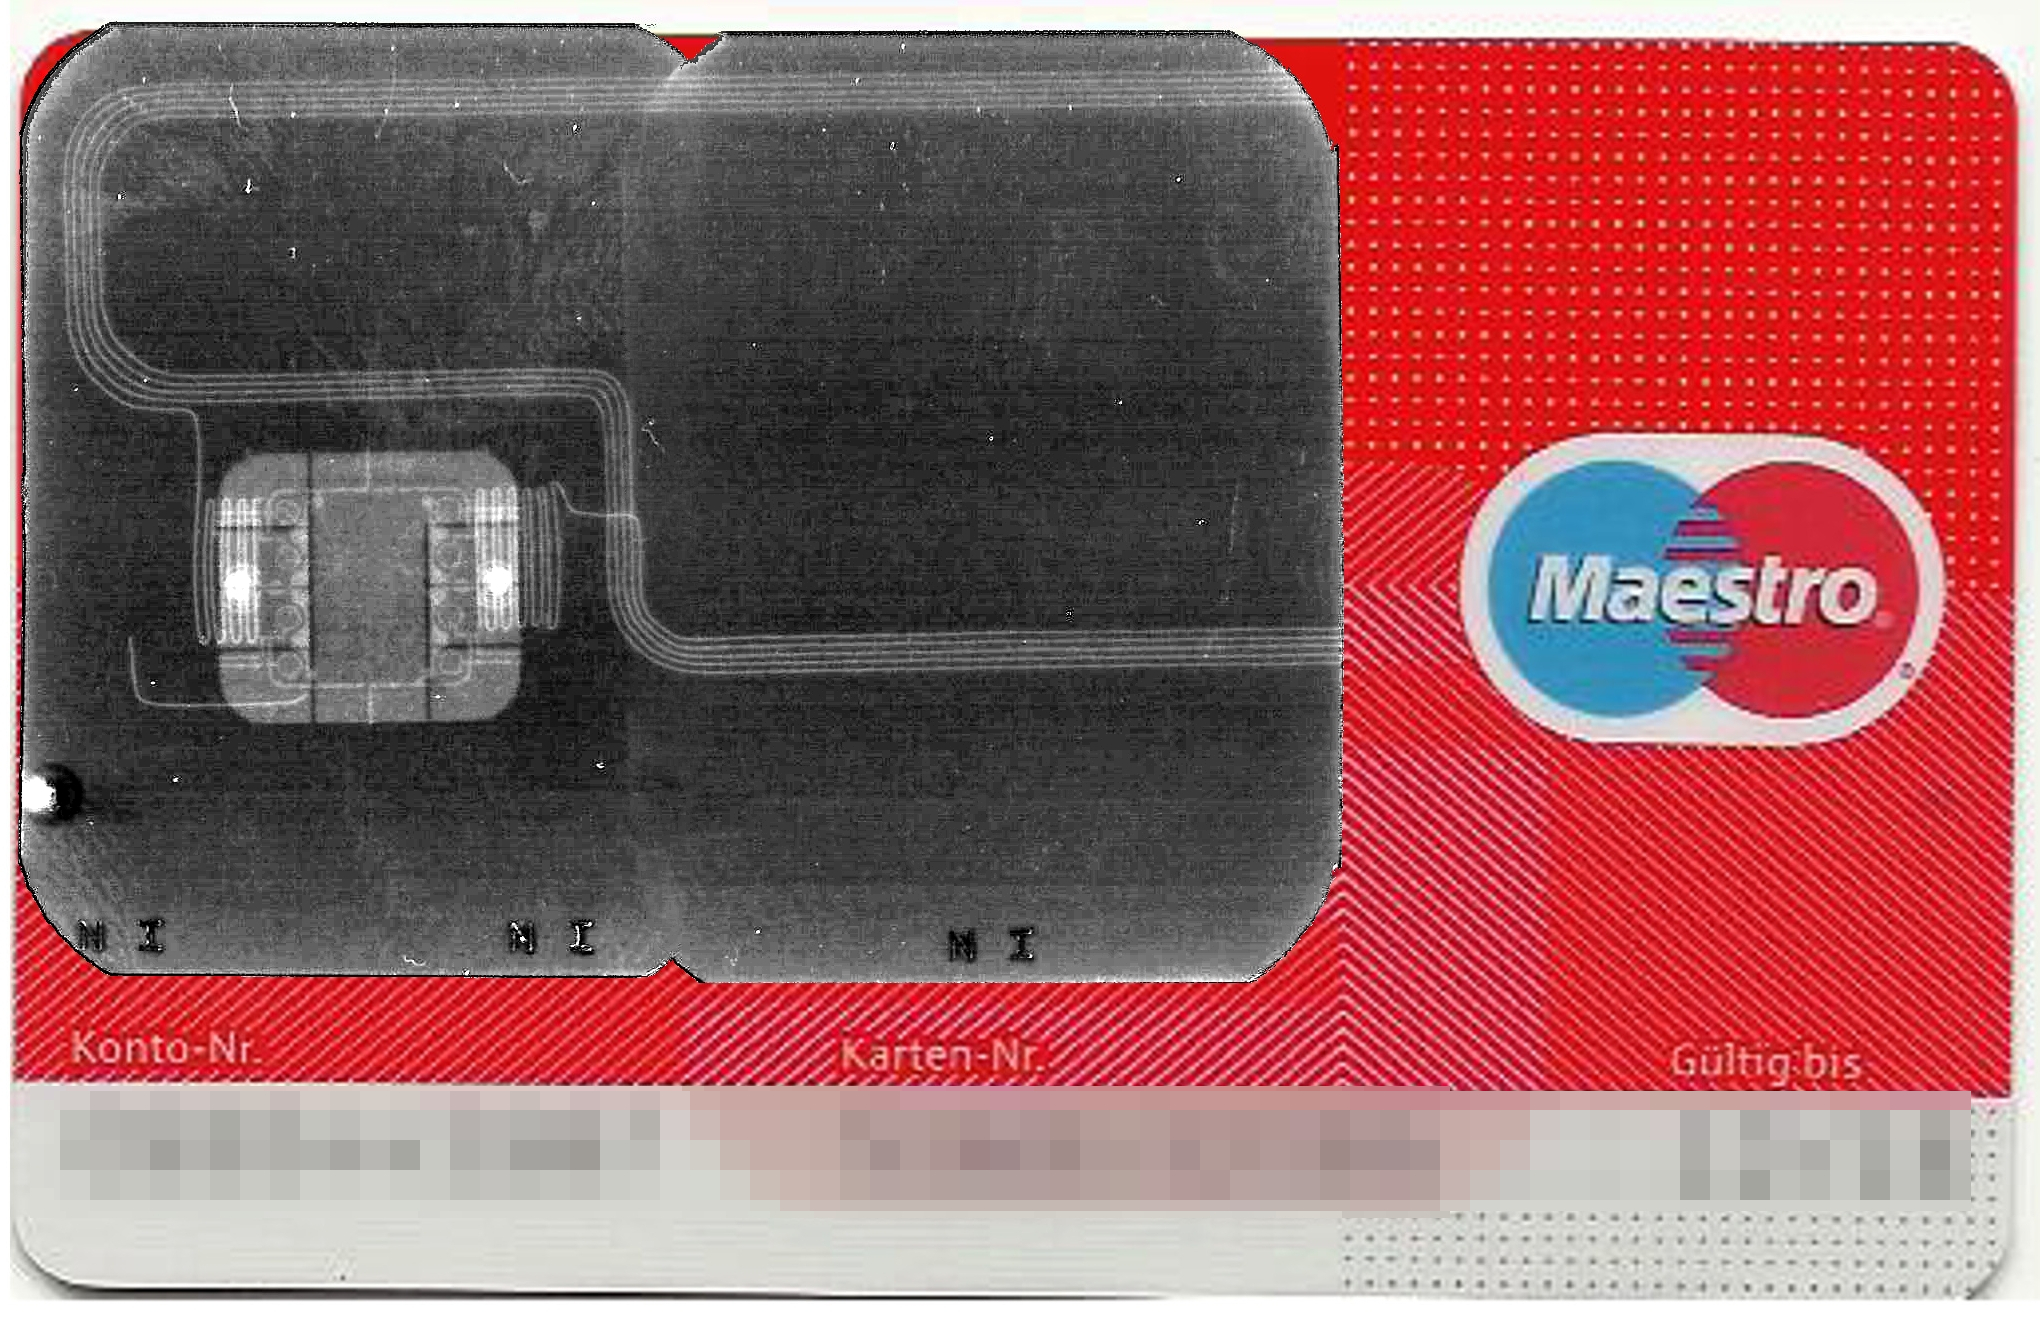
\includegraphics[width=\linewidth]{Kapitel/NFC/Grafiken/girogo.jpg}
\captionof{figure}{Röntgenbild einer Girocard~\cite{nfc.1}}
\label{fig:nfc.girogo}
\end{Figure}

Bei modernen Multimedia Systemen ist NFC häufig bei Vorhandensein einer Bluetooth Funktion anzutreffen, um ein schnelles und kontaktloses Pairing mit einem anderen Bluetooth Gerät zu ermöglichen.~\cite{nfc.2,nfc.11,nfc.12}


\subsection*{Ausblick}
Als Studentenausweis mit Bezahlfunktion oder Schlüsselersatz für Mitarbeiter hat sich NFC bis heute nicht durchgesetzt, da hier die ältere RFID Technologie bereits weit verbreitet im Einsatz ist. Während der Übertragungsstandard im Mobile Payment mit Anbietern wie Google Wallet noch ein Nischendasein fristet, bieten die neuen Kreditkarten von Visa (payWave) und MasterCard (PayPass) bereits die Möglichkeit per NFC zu bezahlen. Bis dato unterstützen allerdings nur wenige Händler diese Zahlungsmöglichkeit.

In Zukunft wird NFC meiner Meinung nach vermehrt in der Praxis Anwendung finden, wie zum Beispiel das Ersetzen von Bezahlmitteln durch eine virtuelle Bankkarte, die eine Applikation in einem NFC fähigen Smartphone darstellt, oder das Ersetzen von Autoschlüsseln durch NFC fähige Smartphones.~\cite{nfc.2} Weiteres Potential besteht auch in Applikationen, die in Kombination mit sogenannten „NFC Stickern“ verwendet werden. Hierdurch ist es so zum Beispiel möglich NFC als eine Art Informationsvermittler zu verwenden, der Informationen bereitstellt, wenn das Smartphone in Reichweite des Stickers ist.~\cite{nfc.15}

\printbibliography[segment=12,heading=subbibliography]

\end{multicols}
\newpage
